\subsection{Oberflächenwellen}
% Vrettos2017
% Schmidt2017

\begin{frame}
\frametitle{Video}
\begin{center}

\includegraphics[width=0.2\textwidth]{fig_img/youtube.png}   
\end{center}

\href{https://www.youtube.com/watch?v=6yXgfYHAS7c}{\textsl{Wolfram: Propagation of Seismic Waves: Rayleigh waves}}

\href{https://www.youtube.com/watch?v=t7wJu0Kts7w}{\textsl{Wolfram: Propagation of Seismic Waves: Love waves}}

\end{frame}


\begin{frame}
\frametitle{Rayleigh Wellen}
\begin{figure}
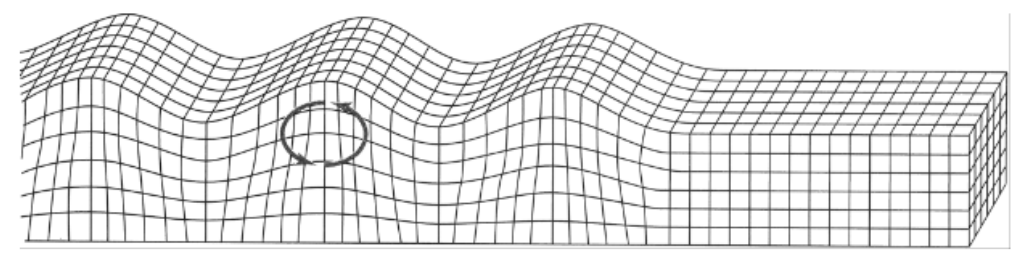
\includegraphics[width=\textwidth]{fig_img/rayleigh_wave} 
\caption*{\cite{Vrettos2017}}
\end{figure}

Beschreibung

\end{frame}


\begin{frame}
\frametitle{Rayleigh Wellen}

\begin{figure}
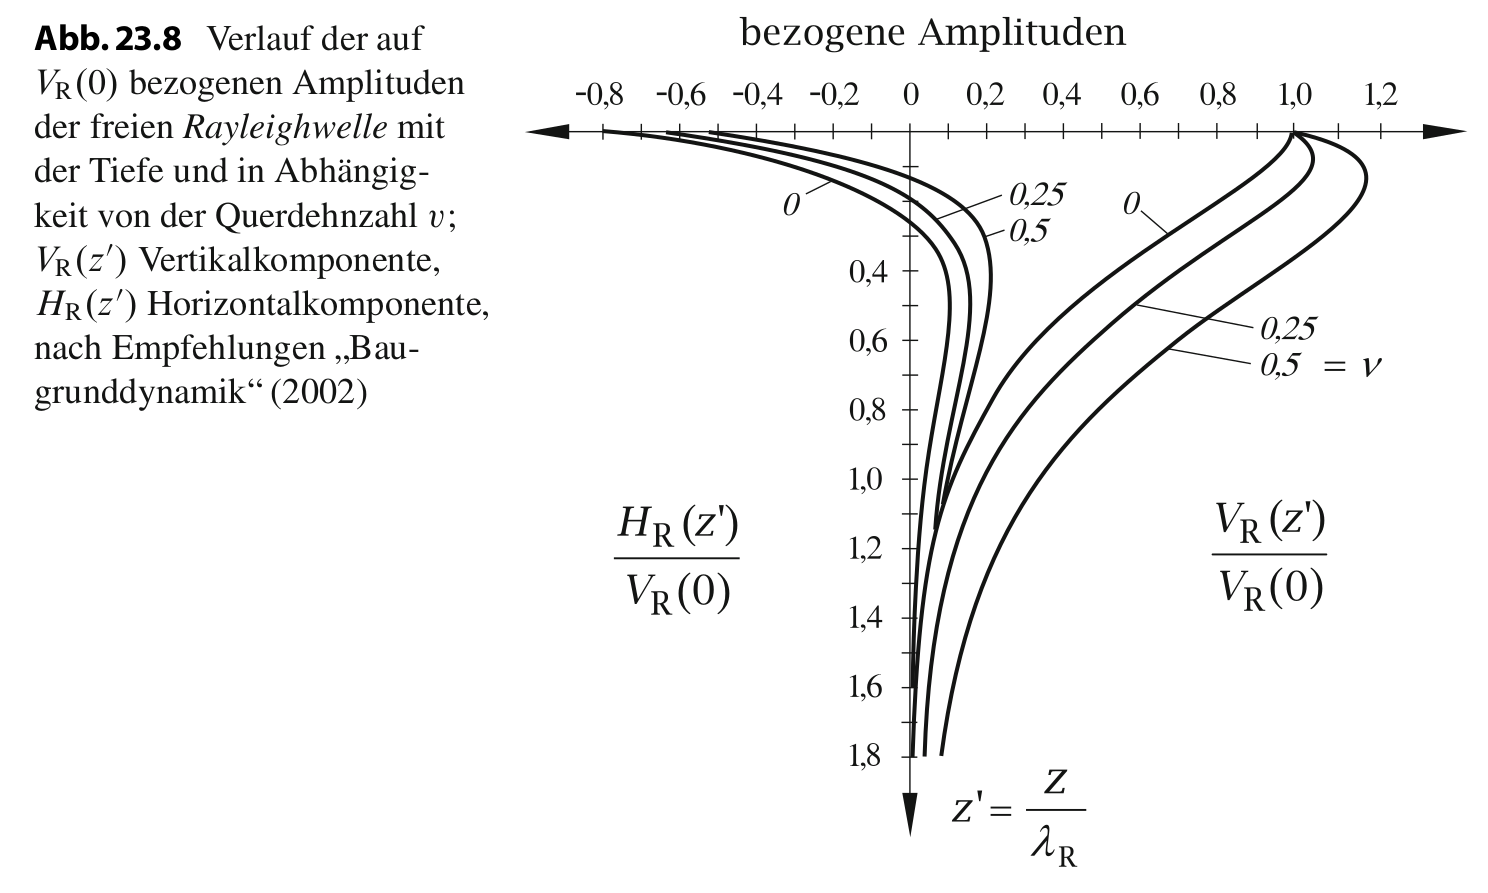
\includegraphics[width=0.8\textwidth]{fig_img/rayleigh_depth} 
\caption*{\cite{Schmidt2017}}
\end{figure}
Dispersion

\end{frame}


\begin{frame}
\frametitle{Kreisfundament}
\begin{figure}
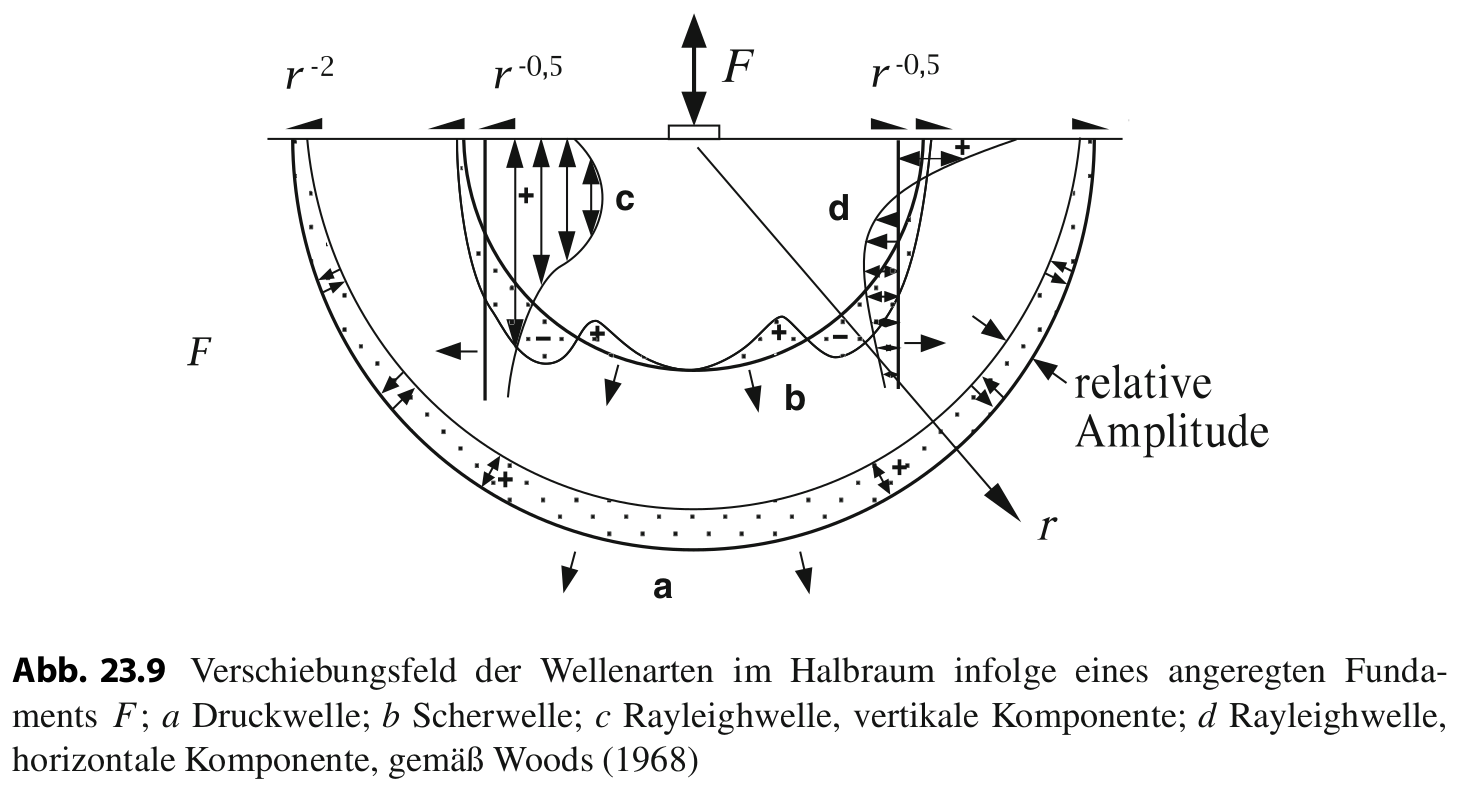
\includegraphics[width=0.9\textwidth]{fig_img/point_load_on_half_space} 
\caption*{\cite{Schmidt2017}}
\end{figure}
Diskussion der Wellen

\end{frame}


\begin{frame}
\frametitle{Love Wellen}
\begin{figure}
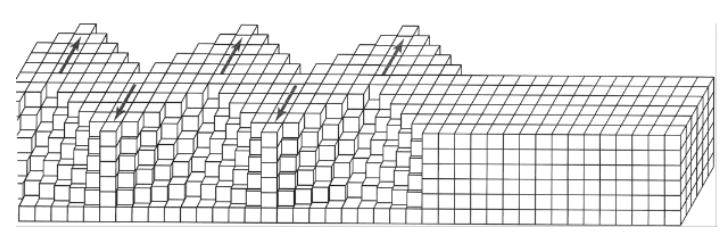
\includegraphics[width=\textwidth]{fig_img/love_wave} 
\caption*{\cite{Vrettos2017}}
\end{figure}
Beschreibung
\end{frame}


\begin{frame}
\frametitle{Erdbeben}
\begin{figure}
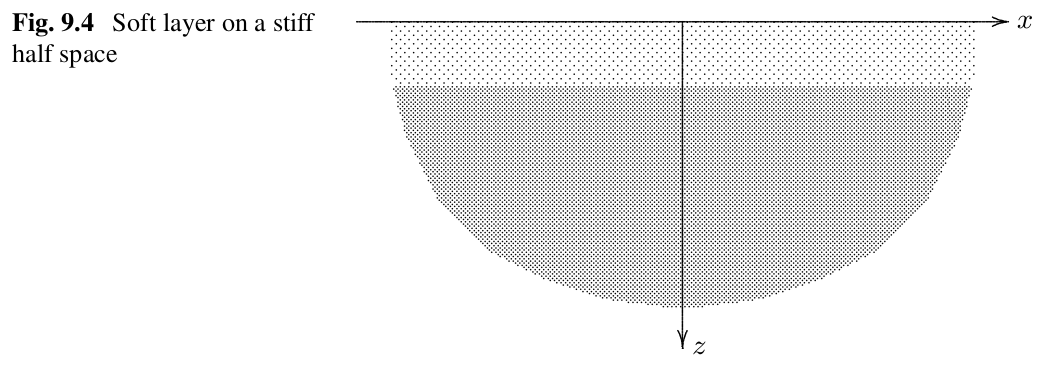
\includegraphics[width=\textwidth]{fig_img/love_wave_configuration} 
\caption*{\cite{Vrettos2017}}
\end{figure}

siehe 1.5D
\end{frame}


